\documentclass{beamer}
\usetheme{Dresden}
%\usetheme{CambridgeUS}
\usepackage{helvet}
\usepackage{cite}
\usepackage{url}
\usepackage{amssymb, amsmath, graphicx, charter, latexsym}
\usepackage{subfigure}
\usepackage{enumerate}
\usepackage{ragged2e}
\usepackage{mathtools}
\usepackage{tabu}
\usepackage{epstopdf}
\usepackage{siunitx}
\renewcommand{\familydefault}{\sfdefault}
%\usepackage{times}
\setbeamertemplate{items}[circle]
\setbeamertemplate{navigation symbols}{}
\begin{document}
\title{Scheduling for Uplink Transmissions with PCF}
\author{Dongni Han, Ping-Chun Hsieh, and Tao Zhao}
\date{March 31, 2016}
\newtheorem{thm}{Theorem} 
\begin{frame}
\titlepage
\end{frame}


%\begin{frame}
%\frametitle{What to Discuss Today?}
%\tableofcontents[]
%\end{frame}

%\AtBeginSection[]
%{
	%\begin{frame}{Table of Contents}
	%\tableofcontents[currentsection]
	%\end{frame}
%}


\section{Introduction}

\begin{frame}
\frametitle{Uplink Transmissions}
\begin{itemize}
\item One AP and N clients
\item 1 slot = 2 RTT; 1 interval = $T$ slots
\item Packets generated in the beginning of each interval
\item Real-time and non-real-time traffic
\end{itemize}
\begin{figure}
\centering
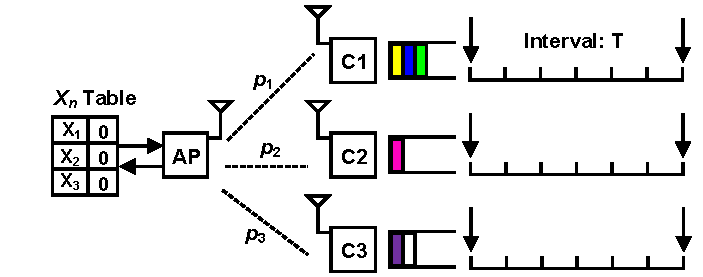
\includegraphics[scale=0.85]{network.pdf}
\end{figure}
\end{frame}

\begin{frame}
\frametitle{Baseline Policy - A Toy Example}
\begin{itemize}
\item Phase 1: AP polls the queue length in a round-robin manner
\end{itemize}
\begin{figure}
\centering
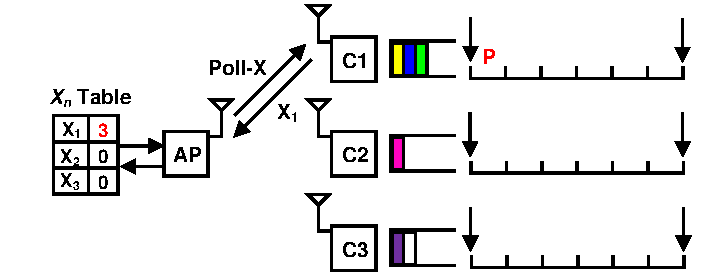
\includegraphics[scale=0.85]{animation_01.pdf}
\end{figure}
\end{frame}

\begin{frame}
\frametitle{Baseline Policy - A Toy Example}
\begin{itemize}
\item Phase 1: AP polls the queue length in a round-robin manner
\end{itemize}
\begin{figure}
\centering
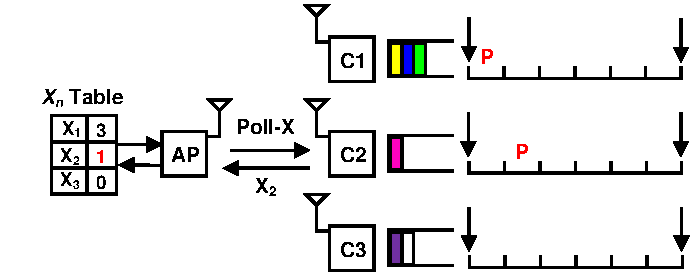
\includegraphics[scale=0.85]{animation_02.pdf}
\end{figure}
\end{frame}

\begin{frame}
\frametitle{Baseline Policy - A Toy Example}
\begin{itemize}
\item Phase 1: AP polls the queue length in a round-robin manner
\end{itemize}
\begin{figure}
\centering
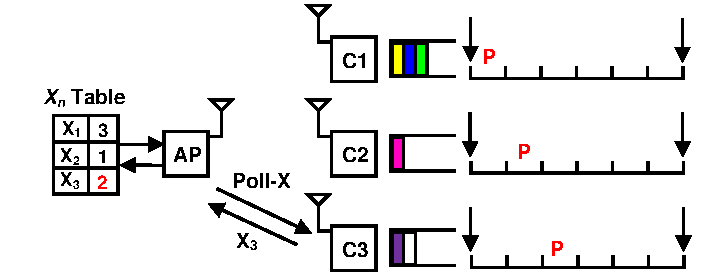
\includegraphics[scale=0.85]{animation_03.pdf}
\end{figure}
\end{frame}

\begin{frame}
\frametitle{Baseline Policy - A Toy Example}
\begin{itemize}
\item Phase 2: AP schedules a client based on Max-Weight policy
\end{itemize}
\begin{figure}
\centering
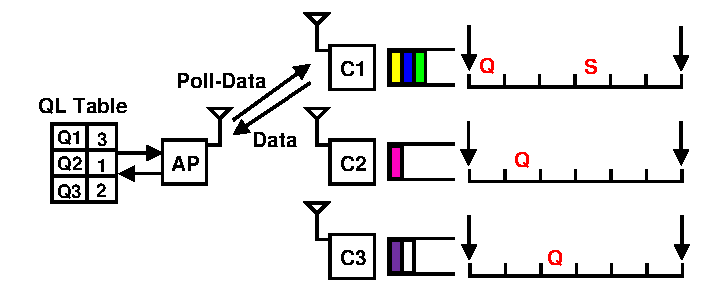
\includegraphics[scale=0.85]{animation_04.pdf}
\end{figure}
\end{frame}

\begin{frame}
\frametitle{Baseline Policy - A Toy Example}
\begin{itemize}
\item Phase 2: AP schedules a client based on Max-Weight policy
\end{itemize}
\begin{figure}
\centering
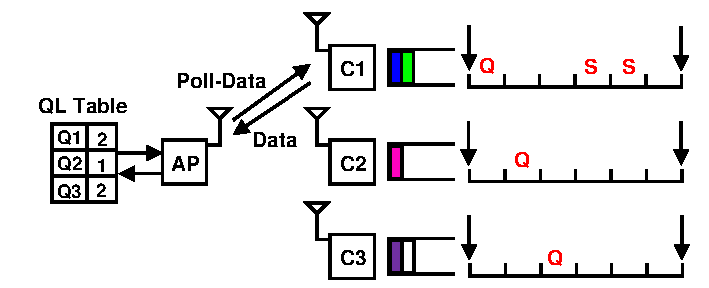
\includegraphics[scale=0.85]{animation_05.pdf}
\end{figure}
\end{frame}

\begin{frame}
\frametitle{Baseline Policy - A Toy Example}
\begin{itemize}
\item Phase 2: AP schedules a client based on Max-Weight policy
\end{itemize}
\begin{figure}
\centering
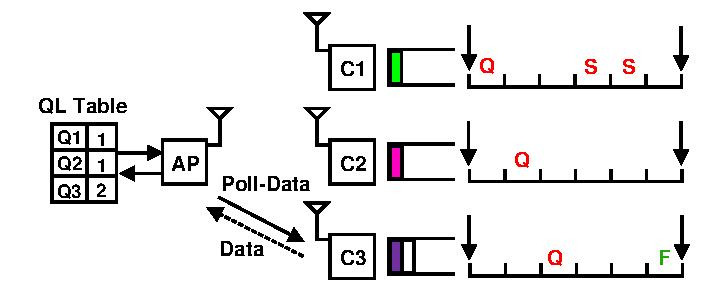
\includegraphics[scale=0.85]{animation_06.pdf}
\end{figure}
\end{frame}


\end{document}
